\chapter{文件与文件管理}
\label{cha:file-and-file-management}

\begin{intro}
  一直以来,「文件管理」都是困扰着许多电脑用户,尤其是初学者的一大难题。看完本章,你将可以找到下面这些问题的答案:
  \begin{itemize}
    \item C 盘、D 盘都是什么?为什么有人建议把软件装到 D 盘里?电脑空间总是不够用,怎么办?
    \item 「扩展名」是什么?「打开方式」又是什么?为什么有时候我电脑上的 Word 文档突然打不开了?
    \item 我应该如何管理好自己的文件?
  \end{itemize}
\end{intro}

如\chapref{cha:computer-and-its-components}一章所言,硬盘是电脑中存放数据的地方,而「文件」则是数据存放的具体形式。你所撰写的 Word 文档、制作的 PowerPoint 幻灯片、从网上下载的图片和视频,乃至各个软件本身,都以文件的形式存储在硬盘上。

本章,我们将具体介绍「文件」以及文件的管理。这是《你缺计课》中需要动手实践的第一章,更是我们合理、有效地使用电脑的第一课。

\section{硬盘的分区}

双击桌面上的【此电脑】,就能打开「\regcolor{文件资源管理器}」,简称「\regcolor{资源管理器}」。在其中,我们可以看到一个或几个「盘」,例如 C 盘、D 盘等。这样的「盘」学名叫做「分区」,顾名思义,它们是将硬盘上的空间人为地划分成了一些子空间。

\begin{note}
  如果你的电脑上没有【此电脑】图标,请先按\chapref{cha:computer-and-its-components}中的方法让它显示在桌面上。
\end{note}

\begin{figure}[htb!]
  \centering
  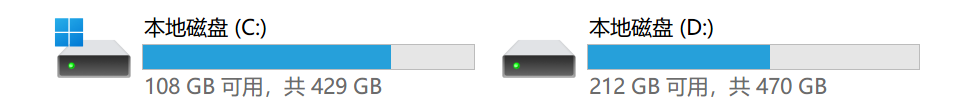
\includegraphics[width=.8\textwidth]{assets/basic/Partitions.png}
  \caption{电脑上的两个分区}
  \label{fig:Partitions1-2}
\end{figure}

例如,上图是一台电脑「文件资源管理器」中显示的分区。可以看到,这两个分区一个大小为 429 GB,另一个大小为 470 GB,相加为 899 GB——这是这台电脑的硬盘可用总空间。

划分分区的意义,在于帮助我们更好地管理文件。分区划分之后,各个分区之间就仿佛被隔离开来了。即使我们「格式化」一个分区(这样会删除这个分区中的所有文件),也不会影响另外一个分区里面的文件。

\begin{figure}[htb!]
  \centering
  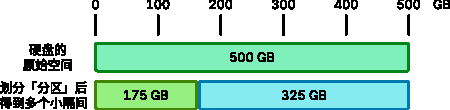
\includegraphics[width=.9\textwidth]{assets/basic/Partition_structure.pdf}
  \caption{分区的结构}
  \label{fig:Partition_structure}
\end{figure}

在 Windows 系统中,分区会被给予两个标识符,或者说「名字」:

\begin{itemize}
  \item 一个是「\regcolor{盘符}」,盘符是一个英文字母加上冒号 \MissingVerb{:} 构成的。我们所称呼的「C 盘」「D 盘」正是指盘符中的那个字母。如上图,左方分区的盘符是 \MissingVerb{C:} ,右方分区的盘符是 \MissingVerb{D:} 。盘符一般在被指定之后就不方便更换了。如今的 Windows 系统中,我们使用的盘符都是从字母 C 开始\footnote{这是因为 A 和 B 两个盘符在过去是留给「软盘」的,但软盘早就已经成为历史了,不过这个习惯却保留了下来。}的。
  \item 另一个是「\regcolor{卷标}」,这是一个可选的标识符,它是一定长度的文本。上图中的 C 盘,卷标就是「本地磁盘」。盘符的作用是让系统和软件识别分区,而卷标的作用是帮助我们用户更加直观地了解分区的作用,因而卷标是可以随时更换的。事实上,通过右键某一分区,选择【重命名】,就可以更换卷标了。如果你什么都不写,它默认显示成「本地磁盘」。
\end{itemize}

\begin{figure}[htb!]
  \centering
  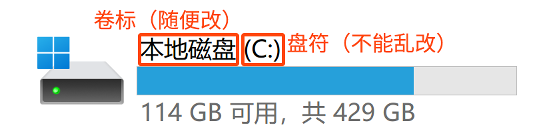
\includegraphics[width=.5\textwidth]{assets/basic/Partition_labels.png}
  \caption{盘符与卷标}
  \label{fig:Partition_labels}
\end{figure}

我们在\chapref{cha:computer-and-its-components}中提到,操作系统本身也是一个大软件,那么这个软件放在硬盘上的哪呢?对于 Windows 而言,\regcolor{整个 Windows 系统默认放在 C 盘里}。双击打开电脑 C 盘,你会看到一些你可能不熟悉的文件夹,例如 \MissingVerb{Windows} 文件夹,Windows 系统自己的许多文件就存在其中。

也许你曾经听过「不要把软件安装到 C 盘」「不要把自己的数据放在 C 盘」这样的说法。这种说法是有一定道理的:如果你的 C 盘总空间较小(这在以前是很常见的情况),而 Windows 系统本身就很庞大,且系统自身工作产生的一些文件也会被自动地放在 C 盘内,这导致 C 盘本身空间很容易变得局促。这时,如果我们还将大量的软件装在 C 盘,就会让 C 盘更加不堪重负,结果就是——满了。

在本章的后续部分,以及\chapref{cha:software-installation}中,我们会详细介绍我们如何比较妥善地利用各个分区。如果你的 C 盘空间已经不足,那么请参考\chapref{cha:manage-storage}中的方法,来释放 C 盘的空间。

\begin{note}
  如果你打开「此电脑」之后,发现自己电脑上只有一个 C 盘,这说明你的电脑磁盘只有一个分区。一些品牌的新电脑出厂时就是这样的设置。如果你想要在 C 盘之后分出一个新的分区,可以参考\chapref{cha:new-laptop-setup}中的方法。如果前面的方法不行,或者你想进行更高级的分区调整(例如调整大小),则需要参见进阶篇的\chapref{cha:manage-storage}。
\end{note}

\section{文件、文件名和文件类型}

\begin{wrapfigure}[5]{r}{7.2cm}
  \centering
  \vspace*{-3ex}
  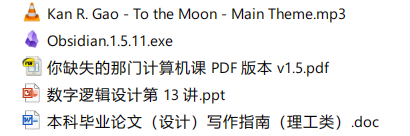
\includegraphics[width=7cm]{assets/basic/5_files.png}
  \caption{一些文件}
  \label{fig:5_files}
\end{wrapfigure}

「文件」是数据存储在硬盘上的形式。这么说可能有些抽象,直观地说,文件就是我们在资源管理器里看到的,像\autoref{fig:5_files} 里面的这些东西。

文件有自己的名字,称为「文件名」。在 Windows 系统中,文件名可以分成三个部分:

\begin{itemize}
  \item 「主名」是指文件名中,「点号」之前的部分。这部分内容可以自定,相当于人类的姓名。上图中,\MissingVerb{数字逻辑设计第 13 讲} 和 \MissingVerb{Obsidian.1.5.11} 等都是文件的主名。
  \item 「点号」是指文件名中间\regcolor{最后一个} \MissingVerb{.}。
  \item 「扩展名」是指文件名中,点号之后的部分\cprotect\footnote{有时候我们称呼文件的扩展名时也会把点号包含进去。下面两种说法是等价的:
    \begin{itemize}
      \item 某文件的扩展名是 \MissingVerb{txt}。
      \item 某文件的扩展名是 \MissingVerb{.txt}。
    \end{itemize}
  }。扩展名指示文件的类型,它会告诉操作系统,这个文件应该用什么方式来打开。例如,上图中 \MissingVerb{本科毕业论文(设计)写作指南(理工类).doc} 中的 \MissingVerb{doc} 就是这个文件的扩展名,它说明这个文件是一个 Word 文档,应该使用 Word 或 WPS 等软件打开。
\end{itemize}

\begin{note}
  如果你的电脑上,文件的扩展名没有显示出来(也就是说你只能看到文件的主名),像这样:

  \begin{center}
    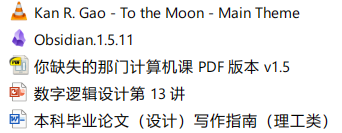
\includegraphics[width=7cm]{assets/basic/5_files_not_showing_extensions.png}
    \captionof{figure}{隐藏扩展名的文件}
    \label{fig:5_files_not_showing_extensions}
  \end{center}

  在 Windows 10 中请点选文件夹窗口上方的【查看】选项卡,然后勾选【文件扩展名】这一项:

  \begin{center}
    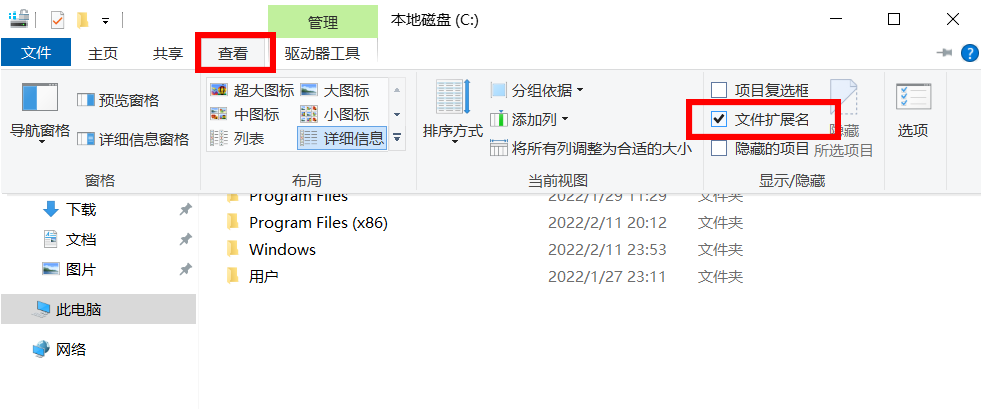
\includegraphics[width=.6\textwidth]{assets/basic/Windows_10_set_full_filename.png}
    \captionof{figure}{在Windows 10中显示文件扩展名}
    \label{fig:Windows_10_set_full_filename}
  \end{center}

  在 Windows 11 中请点选文件夹窗口上方的【查看】菜单,然后勾选【显示】→【文件扩展名】:

  \begin{center}
    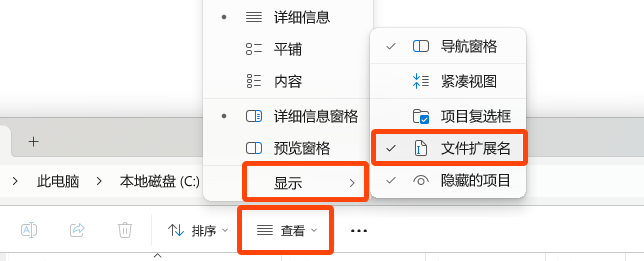
\includegraphics[width=.6\textwidth]{assets/basic/Windows_11_set_full_filename.png}
    \captionof{figure}{在Windows 11中显示文件扩展名}
    \label{fig:Windows_11_set_full_filename}
  \end{center}
\end{note}

扩展名也可以人为改变,但这样往往会出问题——试想,\autoref{fig:5_files} 中的 \MissingVerb{数字逻辑设计第 13 讲.ppt},本来是一个 \MissingVerb{ppt} 文件,即 PowerPoint 幻灯片,应该用 PowerPoint 或 WPS 打开。如果你强行把它改成 \MissingVerb{txt},系统就会用记事本来打开一个幻灯片——用错误的工具打开文件。因此,扩展名不能随便改,因为改了之后系统就会用错误的工具去打开它。右键某一文件,选择【重命名】,你会看到系统会自动帮你选中文件的主名,而不选中扩展名。如果你执意更改文件的扩展名,系统会发出一个提示:

\begin{figure}[htb!]
  \centering
  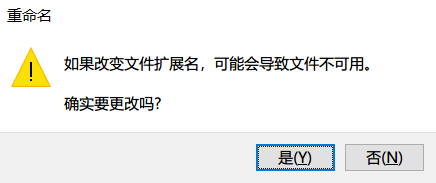
\includegraphics[width=6cm]{assets/basic/Warning_when_changing_extension.png}
  \caption{尝试更改扩展名……}
  \label{fig:Warning_when_changing_extension}
\end{figure}

「那既然这样,我不想不小心突然间改掉文件的扩展名,还不如让扩展名不显示呢。」如果你有这样的想法,那么另一重危险正悄然降临。且看下面的两个文件:

\begin{figure}[htb!]
  \centering
  \begin{minipage}{.48\textwidth}
    \centering
    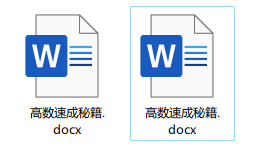
\includegraphics[width=.9\textwidth]{assets/basic/fake_doc.png}
    \caption{两个同名文件?!}
    \label{fig:fake_doc}
  \end{minipage}
  \begin{minipage}{.48\textwidth}
    \centering
    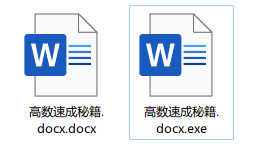
\includegraphics[width=.9\textwidth]{assets/basic/fake_doc_revealed.png}
    \caption{揭示扩展名后}
    \label{fig:fake_doc_revealed}
  \end{minipage}
\end{figure}

这两个「高数速成秘籍」看起来完全一样,就是两个正常的 Word 文档,但众所周知,一个目录下不可能存在两个文件名相同的文件,显然这里面必然有猫腻。现在打开文件扩展名,这两个文件的名称变成了下面这个样子,可见,其中一个居然是可执行文件(\MissingVerb{exe})格式,即一个应用程序(详见下文),只是图标故意被做成了 Word 文档的样子。所以,看不到扩展名的话,指不定哪天有居心叵测的人发来一个这样伪装的病毒,那可就不好了。

\section{文件夹、路径和目录}

「文件夹」是一个用来存放其他文件的结构。不妨想象一下现实中的文件夹:在一个文件夹中,可以放很多各类文件。而电脑中的文件夹除了能放文件之外,还可以放很多的「子文件夹」,即文件夹里面的文件夹。这个过程可以循环重复,因而一个文件夹的内部结构可以相当错综复杂。

假设在 D 盘里的 \MissingVerb{missing} 文件夹之中,有一个叫做 \MissingVerb{源文件} 的子文件夹,在这个子文件夹中有一个文件叫 \MissingVerb{第三章.docx},我们用这种方式表示这个 \MissingVerb{第三章.docx} 文件在整个电脑中的位置:

\begin{MissingVerbatim}
  D:\missing\源文件\第三章.docx
\end{MissingVerbatim}

这一长串东西可以唯一确定地表示出 \MissingVerb{第三章.docx} 这个文件在电脑中的具体位置,我们把一长串东西称为 \MissingVerb{第三章.docx} 这个文件的「路径」(严格来说叫做「绝对路径」)。不难发现,路径是从分区(也就是「盘」)开始,用反斜杠 \MissingVerb{\} 作为分隔,一级一级文件夹地展开,最后到具体的文件。类似的,不只是文件,文件夹的路径也可以用这样的方式来表示,例如
\begin{MissingVerbatim}
  D:\missing\源文件
\end{MissingVerbatim}
\noindent{}表示的就是 \MissingVerb{源文件} 这个文件夹在电脑中的位置。一个文件或文件夹的路径是唯一确定的;一个路径也能唯一确定一个文件或文件夹。

也许你有听说过「目录」这个名字。其实「目录」就是文件夹。例如说「打开目录 \MissingVerb{D:\missing\public}」指的就是打开 D 盘中 \MissingVerb{missing} 文件夹里的 \MissingVerb{public} 文件夹。

目录(文件夹)一层一层的结构可以像\autoref{fig:Tree} 这样从上到下画出来,称作「目录树」。树的特点是从一个「根」开始,生长出许多的枝叶,这和文件夹「一层套一层」的结构是一致的。下图便展示了一棵目录树,它的根是文件夹 \MissingVerb{Documents},而其他的文件和文件夹则是它的枝叶。与现实中的树不同的是,目录树是倒着的,根在上,叶子在下。

\begin{figure}[htb!]
  \centering
  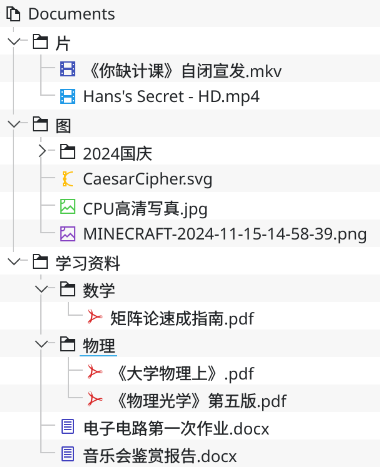
\includegraphics[width=.5\textwidth]{assets/basic/Tree.png}
  \caption{目录树}
  \label{fig:Tree}
\end{figure}

在目录树这种形式中,文件夹之间是「上下级」的关系,故「文件 A 在文件夹 B 中」也可以称作「文件 A 在文件夹 B 下」或者「A 在目录 B 下」甚至是「A 在 B 下」。也就是说,「下」这个字就是「在……里」的意思。

借助目录树这样的结构,我们就能理解「根目录」这个概念了。一个盘的「根目录」就指的是这个盘本身那一级目录——恰好是目录树的根,例如 C 盘根目录就指的是路径 \MissingVerb{C:\} 。

\section{程序本身——可执行文件(\MissingTT{exe} 文件)}

\begin{wrapfigure}{r}{5.2cm}
  \centering
  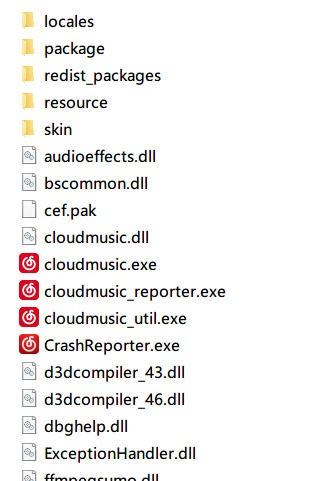
\includegraphics[width=5cm]{assets/basic/NCM_directory.png}
  \caption{网易云音乐的目录}
  \label{fig:NCM_directory}
\end{wrapfigure}

这一节我们介绍一种类型特殊的文件——「可执行文件」。我们提到,数据是以文件的形式存储在硬盘上的,比如你所撰写的 Word 文档,它们都存储成了扩展名为 \MissingVerb{doc} 或者 \MissingVerb{docx} 的文件;你所下载的图片,它们的扩展名则往往是 \MissingVerb{jpg} 、 \MissingVerb{png} 或者 \MissingVerb{gif} 。而我们又提到,软件也是以文件的形式存储在硬盘上的。那么,软件本身是什么格式的文件呢?

一个软件的核心是一个或多个「程序」,而程序是以「可执行文件」的形式存储的。\regcolor{普通的文件,需要用其他的某个软件才能正常打开;而「可执行文件」双击就能运行自身,这就是「可执行」(Executable)的意思。}

可执行文件的扩展名是 \MissingVerb{exe} 。对于这种类型的文件,系统不会想着用别的软件去打开它,而是直接运行它自身。可执行文件有时被直接称为「程序文件」或者「程序」。

需要注意的是,电脑上的一款软件可能不是仅仅只有一个 \MissingVerb{exe} 文件。例如,右图是软件「网易云音乐」所在的文件夹中的一部分。

可以看到,网易云音乐有着这些文件:

\begin{itemize}
  \item 可执行文件 \MissingVerb{cloudmusic.exe} ,这个是「网易云音乐」的主程序。
  \item 可执行文件 \MissingVerb{cloudmusic_reporter.exe},\MissingVerb{cloudmusic_util.exe} 等。这些文件是软件运行时的其他辅助程序。它们往往无法单独运行,而 \MissingVerb{cloudmusic.exe} 这个主程序脱离它们也不能正常运行。
  \item 一大堆的 \MissingVerb{dll} 和其他格式的文件。这些是软件工作时不可或缺的依赖文件。
  \item 一些子文件夹,存储着软件运行需要的一些资源。
\end{itemize}

每次我们启动网易云音乐,运行的都是 \MissingVerb{cloudmusic.exe} 这个可执行文件。然而,这个文件的运行离不开放在它边上的那一堆辅助文件——如果你把 \MissingVerb{cloudmusic.exe} 复制到另外的一个地方,双击运行,大概率会直接报错;即使不报错,功能也必不完全正常。在后续的章节,我们在介绍软件的安装与卸载时,会继续提到这件事。

\begin{note}
  好奇这 \MissingVerb{exe} 文件里面到底是什么?答案将在超越篇的\chapref{cha:program-and-arch} 揭晓。
\end{note}

\section{文件的「替身」——快捷方式}

你是怎么启动网易云音乐的呢?

一般来说,我们会双击桌面上的「网易云音乐」,或者点击开始菜单中的「网易云音乐」。然而,这些地方看到的「网易云音乐」,都不是这个软件的本体,而是另一种称为「快捷方式」的特殊文件。「快捷方式」可以看成某个具体文件的单向「指针」或者说「替身」,打开快捷方式就相当于打开了本体。

\begin{figure}[htb!]
  \centering
  
\includegraphics[width=10cm]{assets/basic/Link.pdf}
  \caption{快捷方式}
  \label{fig:Link}
\end{figure}

快捷方式的扩展名是 \MissingVerb{lnk},但实际上不可见\cprotect\footnote{千万不要手动把一个正常文件的扩展名改成 \MissingVerb{lnk},否则就很难改回来了。}。我们桌面上的「网易云音乐」,指向的正是网易云音乐软件目录下的那个 \MissingVerb{cloudmusic.exe} 文件。右击桌面上的【网易云音乐】,选择【属性】,会弹出这个快捷方式的详细信息,如\autoref{fig:Link_properties} 所示。

\begin{wrapfigure}[12]{r}{6cm}
  \centering
  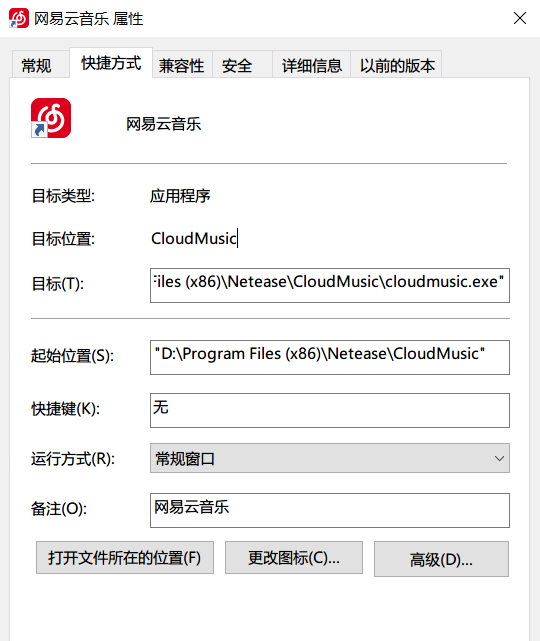
\includegraphics[width=5.8cm]{assets/basic/Link_properties.png}
  \caption{「网易云音乐」的快捷方式}
  \label{fig:Link_properties}
\end{wrapfigure}

其中「目标」一栏填写的正是 \MissingVerb{cloudmusic.exe} 这个可执行文件,即「网易云音乐」的主程序的路径:

\begin{MissingVerbatim}
  D:\Program Files (x86)\Netease\CloudMusic\cloudmusic.exe
\end{MissingVerbatim}

因此,双击打开这个「网易云音乐」快捷方式,就等同于打开 \MissingVerb{cloudmusic.exe} 这个文件。\cprotect\regcolor{如果你删掉了这个快捷方式,它并不会影响 \MissingVerb{cloudmusic.exe} 这个文件,不会影响你电脑上安装的网易云音乐本身。}因此,卸载软件并非仅仅把桌面上的「快捷方式」删掉就完事了,而是需要通过借助卸载工具。我们将在\chapref{cha:basic-maintenance}中介绍。

所有类型的文件以及文件夹都可以制作无数个快捷方式。如果你想给自己的某个文件/文件夹制作一个快捷方式,只需右键它,选择【发送到】→【桌面快捷方式】,就能在桌面生成一个指向这个文件的快捷方式了。这个快捷方式可以挪到系统的任何地方,也可以复制粘贴出很多个副本。它们全都指向原来的那个文件本身。

一般来说,快捷方式的图标左下角会有一个「↗」符号。这个符号标志着这个文件并非某文件本身而是一个快捷方式。

\section{合多为一,精简空间——压缩文件}

「压缩文件」又称「压缩包」,是一种常用的文件类型。人们可以\regcolor{利用「压缩工具」这种软件,将一批松散的文件和文件夹「打包」成一个压缩文件}\footnote{也可以打包成多个文件,称为「分卷压缩」,详见\chapref{cha:archive-formats-and-tools}一章。}。假设你有 8 个文件夹以及 7 个文件一共 15 个项目,你想一次性把它们分享给别人,那么把它们打包成一个压缩文件不失是一种好的选择。

\begin{figure}[htb!]
  \centering
  
\includegraphics[width=.7\textwidth]{assets/basic/Compress_and_decompress.pdf}
  \caption{压缩与解压}
  \label{fig:Compress_and_decompress}
\end{figure}

压缩文件有很多种类,常见的有 \MissingVerb{zip} 文件和 \MissingVerb{rar} 文件,但后者的压缩软件是收费的\cprotect\footnote{具体来说,大多数压缩工具都可以解压 \MissingVerb{rar} 格式的压缩包,但只有 WinRAR 这一款压缩工具可以制作这种格式的压缩包;而这款工具是收费的。详见\chapref{cha:archive-formats-and-tools}。}。我们建议在与他人交换文件的时候,使用\MissingVerb{zip} 格式打包。

当收到一个压缩文件时,我们一般需要将它解压,来还原出原始的文件。如果你电脑上已经安装有压缩工具,那么可以右击压缩文件,选择类似「解压到当前文件夹」\footnote{部分压缩工具称「解压」为「提取」,而有的压缩工具称「解压到此处」,它们的意思是一样的。}或者「解压到 \MissingVerb{<文件名>\}」的选项。这两类选项的不同是:

\begin{itemize}
  \item 「解压到当前文件夹」会把压缩文件里的内容直接放在压缩文件的同一目录下。例如,如果一个压缩文件 \MissingVerb{archive.zip} 里面有 \MissingVerb{a.txt} 和 \MissingVerb{b.txt} 两个文件,选择此选项,解压后 \MissingVerb{a.txt} 和 \MissingVerb{b.txt} 都和 \MissingVerb{archive.zip} 在同一级目录。
  \item 「解压到 \MissingVerb{<文件名>\}」会把压缩文件里的内容放在一个子文件夹里面。在上面的例子中选择这个选项,会在 \MissingVerb{archive.zip} 的同一级目录新建一个文件夹 \MissingVerb{archive},然后把 \MissingVerb{a.txt} 和 \MissingVerb{b.txt} 放在 \MissingVerb{archive} 文件夹下。
\end{itemize}

\begin{figure}[htb!]
  \centering
  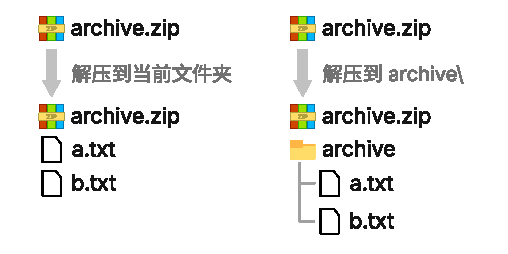
\includegraphics[width=.6\textwidth]{assets/basic/Extract.pdf}
  \caption{不同的解压指令}
  \label{fig:Extract}
\end{figure}

我们建议,为了不让自己的工作目录变得混乱,\cprotect\regcolor{尽量使用「解压到 \MissingVerb{<文件名>\}」}。

\begin{note}
  想想为什么?
\end{note}

如果我们只是想查看一个压缩文件的内容,而不把它解压,可以直接双击打开它,压缩软件会展示出其中的内容。双击这里面的单个文件可以临时取出这一个文件并打开它,拖拽其中的单个文件到其他地方可以只取出这一个文件而不解压整个压缩文件。但是,\regcolor{若你想运行压缩文件中的程序(可执行文件),请一定要完整解压文件},否则程序很可能无法正常工作。

\begin{figure}[htb!]
  \centering
  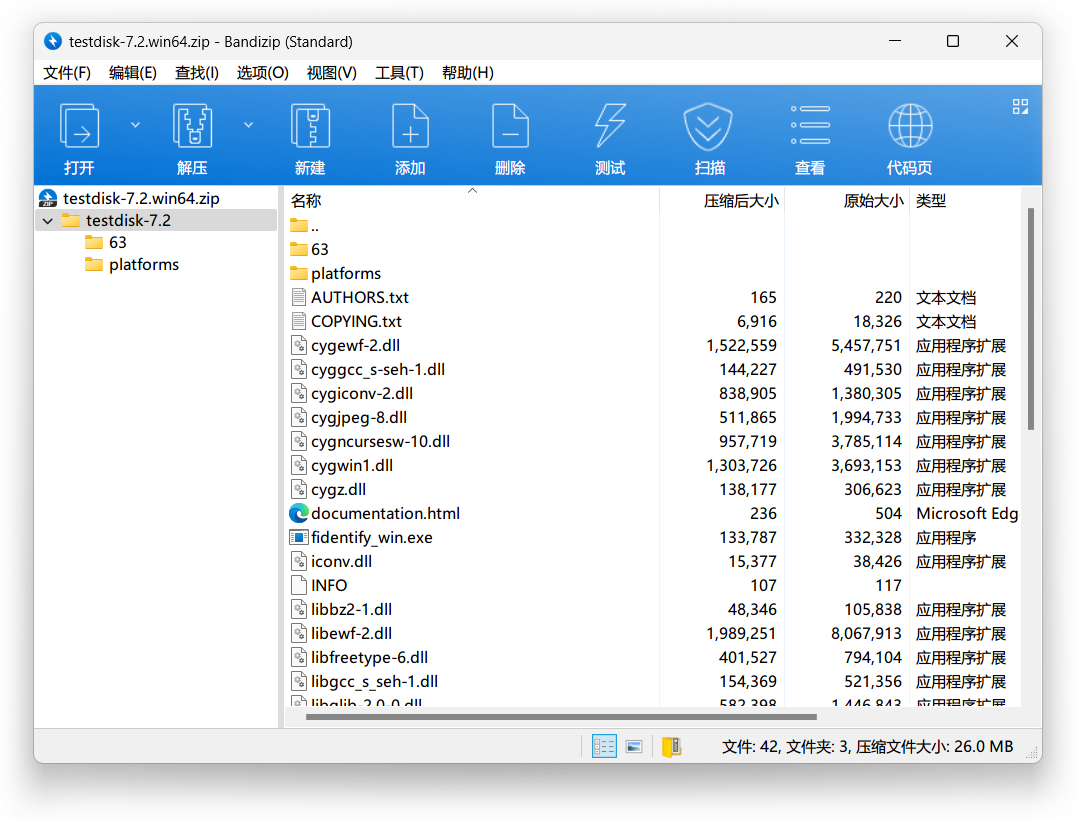
\includegraphics[width=.7\textwidth]{assets/basic/Opened_archive.png}
  \caption{打开一个压缩包}
  \label{}
\end{figure}

当你想制作一个压缩文件时,可以先选中你要打包的所有文件和文件夹,右击它们并选择类似「新建压缩包」或「压缩为 \MissingVerb{<文件名>}」的选项。压缩工具可能会提示你设置一些参数,例如压缩格式(推荐 \MissingVerb{zip} 格式)、压缩后的文件的文件名以及压缩方式。

有关压缩文件和压缩工具的更多细节,请参见本书软件篇的\chapref{cha:archive-formats-and-tools}一章。

\section{文件的打开方式}

在前文中说到,不同类型的文件需要用不同的软件来打开。对于一个特定的文件类型,打开它的软件称为它的「打开方式」。如果打开方式不对,就会出现问题。

容易想到,Word 文档 \MissingVerb{doc} 和 \MissingVerb{docx} 文件的打开方式就是 Word 软件或者 WPS 软件;图片 \MissingVerb{jpg}、 \MissingVerb{png} 等的打开方式就是各种看图软件;PDF 文档 \MissingVerb{pdf} 的打开方式就是 PDF 阅读器,例如 Acrobat 或者 SumatraPDF……

\begin{note}
  可执行文件的打开方式是什么呢?因为它们自己就是程序本身,所以没有「打开方式」的概念。
\end{note}

\begin{table}[htb!]
  \centering
  \caption{神奇的「表」}
  \label{tab:regtable}
  \begin{tblr}{
    colspec = X[.8]X[1.2]X[6.2],
    cells = {c, m},
    cell{2-Y}{Z} = {j},
    row{1} = {fg = white, bg = missing, font = \bfseries},
    row{even} = {MissingSkyBlue},
  }
    \toprule
    扩展名 & 用什么软件打开 & 软件主程序的路径在哪 \\
    \midrule
    \MissingTT{txt} & 记事本 & \MissingTT{C:\textbackslash{}Windows\textbackslash{}system32\textbackslash{}notepad.exe}  \\
    \MissingTT{docx} & Word & \MissingTT{C:\textbackslash{}Program Files\textbackslash{}Microsoft Office\textbackslash{}root\textbackslash{}Office16\textbackslash{}WINWORD.EXE}  \\
    \MissingTT{mp3} & 网易云音乐 & \MissingTT{D:\textbackslash{}Program Files (x86)\textbackslash{}Netease\textbackslash{}CloudMusic\textbackslash{}cloudmusic.exe}  \\
    …… & …… & …… \\
    \bottomrule
  \end{tblr}
\end{table}

系统内部维护有一张「表」,这张表记录了已知的文件类型(扩展名)和对应的打开方式。你可以把这张表想象成\autoref{tab:regtable} 那样。

有了这张表,系统就能自动地帮我们选择文件对应的打开方式。有时,我们不想要用这张表帮我们预置的方式来打开文件。比如,打开 \MissingVerb{png} 图片的默认方式是「照片」软件,但如果我们想\textbf{暂时}用「画图」来打开它,我们可以这样做:

\begin{itemize}
  \item 右键要打开的这个 \MissingVerb{jpg} 文件,选择【打开方式】,在里面选择【画图】,如\autoref{fig:Open_with} 所示。
  \item 如果上一步找不到「画图」,那么选择【打开方式】→【选择其他应用】。然后在弹出的对话框中寻找并点击【画图】。然后,对于 Windows 10,不要勾选【始终使用此应用打开 \MissingVerb{.png} 文件】,直接点击【确定】;对于 Windows 11,点击【仅一次】,如\autoref{fig:Open_with_dialog} 所示。
    \begin{figure}[htb!]
      \centering
      \begin{minipage}{.55\textwidth}
        \centering
        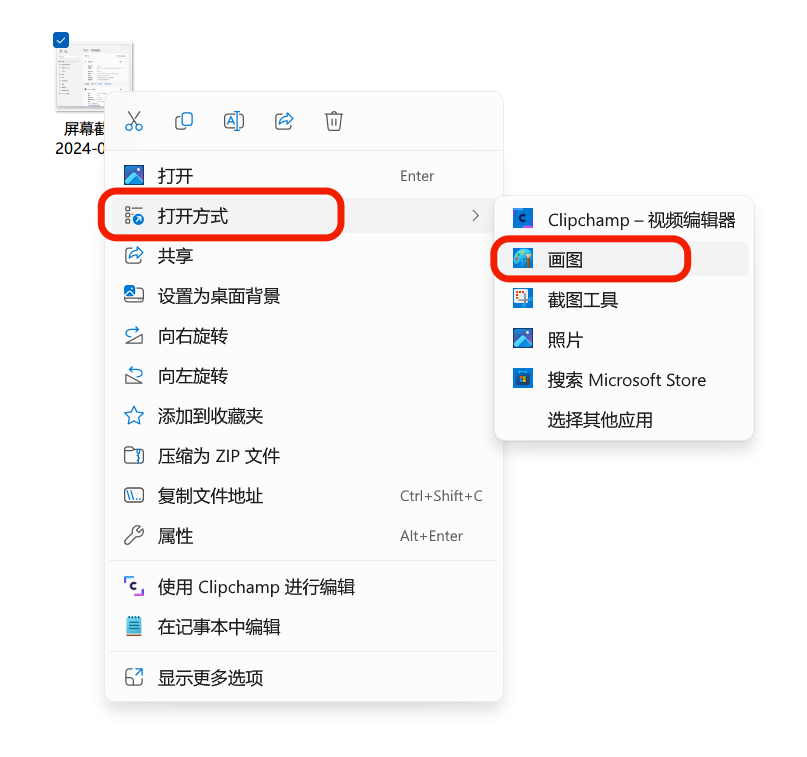
\includegraphics[width=.98\textwidth]{assets/basic/Open_with.png}
        \caption{更改打开方式}
        \label{fig:Open_with}
      \end{minipage}
      \begin{minipage}{.43\textwidth}
        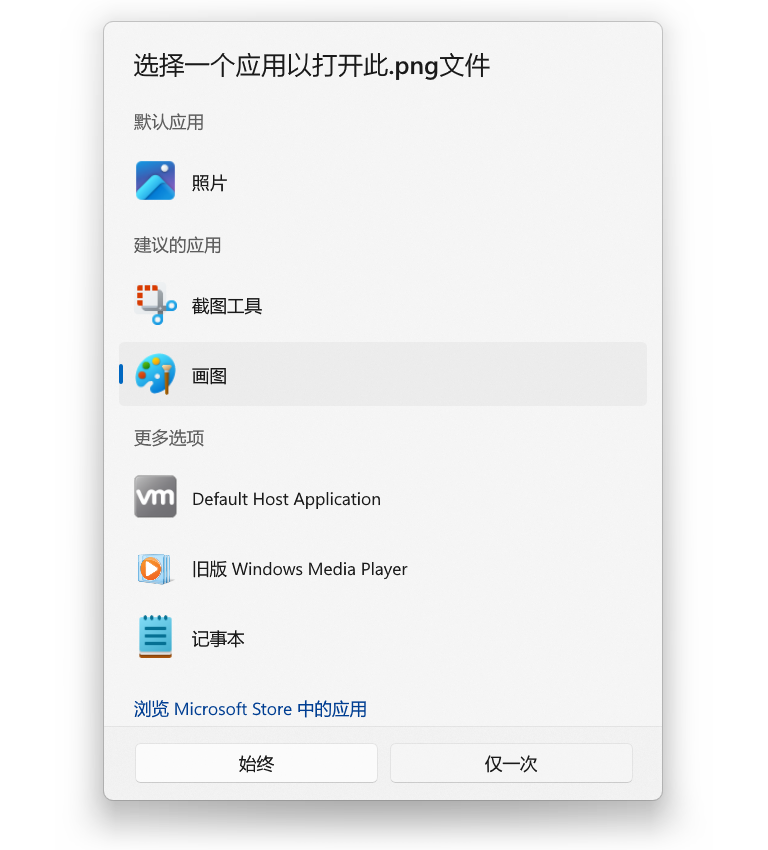
\includegraphics[width=.98\textwidth]{assets/basic/Open_with_dialog.png}
        \caption{选择更多应用}
        \label{fig:Open_with_dialog}
      \end{minipage}
    \end{figure}
  \item 如果你想用自己安装的软件打开这个文件,而上一步的界面找不到那个软件,例如 Adobe Photoshop,那么可能需要手动找到 Adobe Photoshop 的可执行文件,也就是它的 \MissingVerb{exe} 文件。这个文件的路径——也就是软件的安装路径——在下一章我们会提到,一般来说是在 \MissingVerb{C:\Program Files} 或者 \MissingVerb{C:\Program Files (x86)} 之下的某个文件夹中。
\end{itemize}

\regcolor{如果你想永久地指派某一文件的打开方式,则可以在上面步骤的基础上,Windows 11 点击【始终】,Windows 10 则勾选【始终使用此应用打开 \MissingTT{XXX} 文件】。}这样,系统内部的那张表就会被更改,系统以后都会用你指派的新应用来打开这种文件。

除了你手动更改之外,这张表还可能在这些情况被更改:

\begin{itemize}
  \item 系统安装更新,即 Windows 更新之后,这张表可能会被重置而丢失一些项目,造成某些文件突然无法打开。这有可能是由于你使用的对应软件并不是原版,而是某种「精简版」。
  \item 新安装一个软件时,软件安装程序可能写入新的表项,来为即将安装的新软件的文件类型配置打开方式。
  \item Windows 本身的行为。例如,Windows 可能会时不时用 Microsoft Edge 代替其他软件来打开网页文件和 \MissingVerb{pdf} 文件等。\CJKsout*{(微软你坏事做尽)}
\end{itemize}

如果你的文件关联某天突然失效,即某种类型的文件突然无法打开,但对应的软件工作正常,那么可以考虑是否是上面的原因。

\section{管理好你的文件}

管理好我们的文件,不外乎两个方面:

\begin{itemize}
  \item \regcolor{将自己的文件整理归类。}比起将所有文件随手乱放在桌面上,如果我们将自己的文件按它们的性质、类别等归类存放,必然有助于提升我们的工作效率。
  \item \regcolor{妥善利用各个分区,如果可行,尽量不把大量重要文件放在 C 盘。}在前文我们说了,C 盘是 Windows 系统整个所在的地方。如果 C 盘空间本身就有限,在 C 盘存放大量数据会显著增加空间压力。另一方面,尽管发生这种情况的概率很低,但当我们的电脑因为这样或那样的原因损坏,而需要重新安装系统的时候,你会不得不失去 C 盘的所有文件——因为多数时候,我们安装系统的第一步就是格式化 C 盘。
\end{itemize}

\subsection{分区的选择}

取决于你电脑硬盘的大小以及分区的情况,我们推荐了一些方案:

\begin{itemize}
  \item 如果你的电脑只有一个分区——C 盘:
  \begin{itemize}
    \item 若它的总容量小于 300 GB,建议不要再分额外的分区,将你的文件直接存放在 C 盘。同时,你可以使用移动硬盘或各种「网盘」来备份好你的重要数据。
    \item 若它的总容量在 300 GB—500 GB,可以选择为 C 盘留下 200 GB 左右,并将剩余的空间分出一个新的分区(D 盘),然后在 D 盘存放你的文件;当然,你也可以选择不再分额外的分区,将文件直接存放在 C 盘并自行做好备份。
      \begin{note}
        如果你想要在 C 盘之后分出一个新的分区,可以参考本书附录 \chapref{cha:new-laptop-setup}中的方法。如果前面的方法不行,或者你想进行更高级的分区调整(例如调整大小),则需要参见进阶篇的 \chapref{cha:manage-storage}。
      \end{note}
    \item 若它的总容量在 500 GB 以上,建议为 C 盘留出 400 GB—500 GB 的空间,再将剩余的空间按自己的喜好,分出一个或多个新的分区(D 盘、E 盘……)。然后,在这些分区存放你的文件。
  \end{itemize}
  \item 如果你的电脑已经有多个分区(C 盘、D 盘……),可以先在「任务管理器」中,查看每个分区对应的硬盘:
  \begin{itemize}
    \item 若你只有一块硬盘,通常这种情况下,你的 C 盘不会很大,建议直接在 D 盘和之后的分区存放你的文件。
    \item 若你有多块硬盘,并且所有硬盘都是 SSD,我们亦建议你使用 D 盘和之后的分区存放文件。
    \item 若你有多块硬盘,并且有的分区在 SSD 上,有的分区在 HDD 上,我们建议你将常用的软件和数据放在位于 SSD 的分区上(包括 C 盘),而将其他大型软件和不那么常用的数据放在位于 HDD 的分区上。
  \end{itemize}
\end{itemize}

当然,这些方案并非绝对,你可以根据自己的情况选择,适度调整分配大小。

\subsection{为文件安家}

为了给文件安家,我们首先需要挑选一个合适的位置。\regcolor{如果你打算把文件放在 C 盘,可以使用 Windows 为你提供的一系列「已知文件夹」(Known Folder)},即「文档」「视频」「下载」等。

Windows 11 系统中,默认情况下,所有的已知文件夹会被固定在【此电脑】窗口(即资源管理器)的左侧,如\autoref{fig:Win11_user_folders}。

\begin{figure}[htb!]
  \centering
  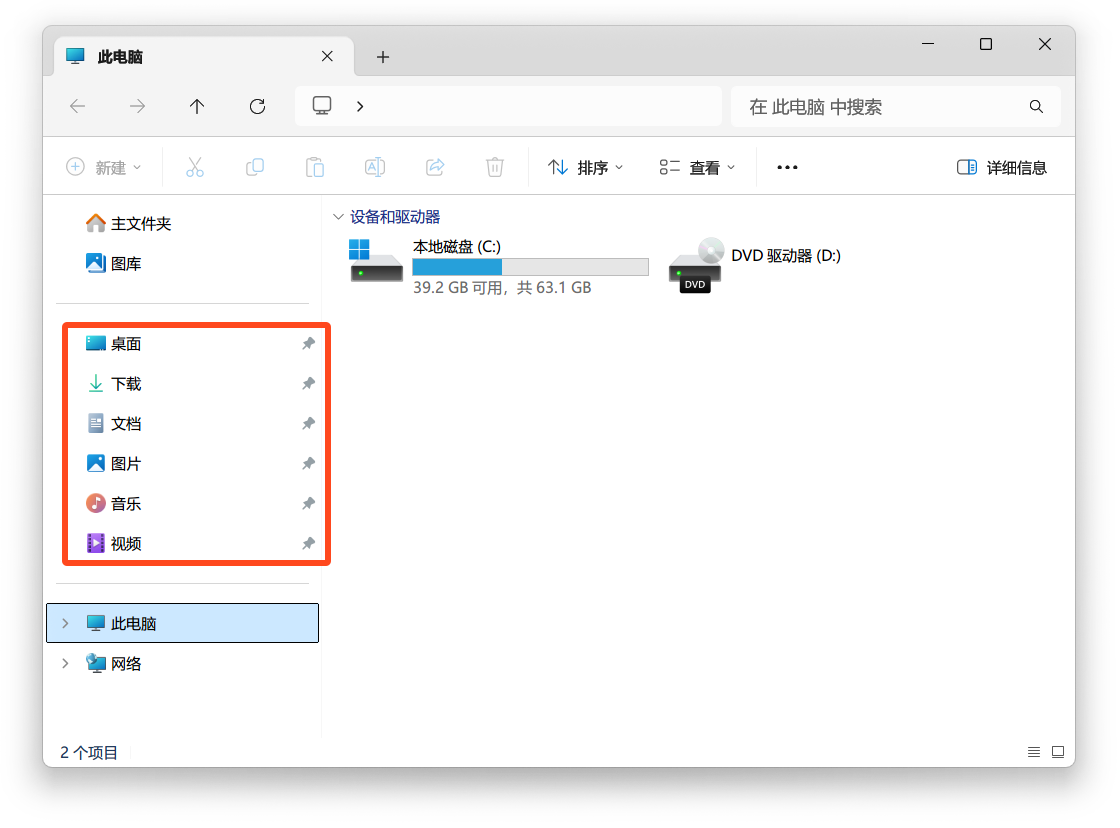
\includegraphics[width=.7\textwidth]{assets/basic/Win11_user_folders.png}
  \caption{Windows 11 的已知文件夹}
  \label{fig:Win11_user_folders}
\end{figure}

如果你在【此电脑】窗口左侧没有看见这些已知文件夹,有可能是它们被不小心解除固定了。为了找到它们,你可以双击资源管理器的地址栏,输入「桌面」两个字并回车,就能看见所有的已知文件夹了。你可以趁此机会右键 →【固定到快速访问】来把它们固定回去。

\begin{figure}[htb!]
  \centering
  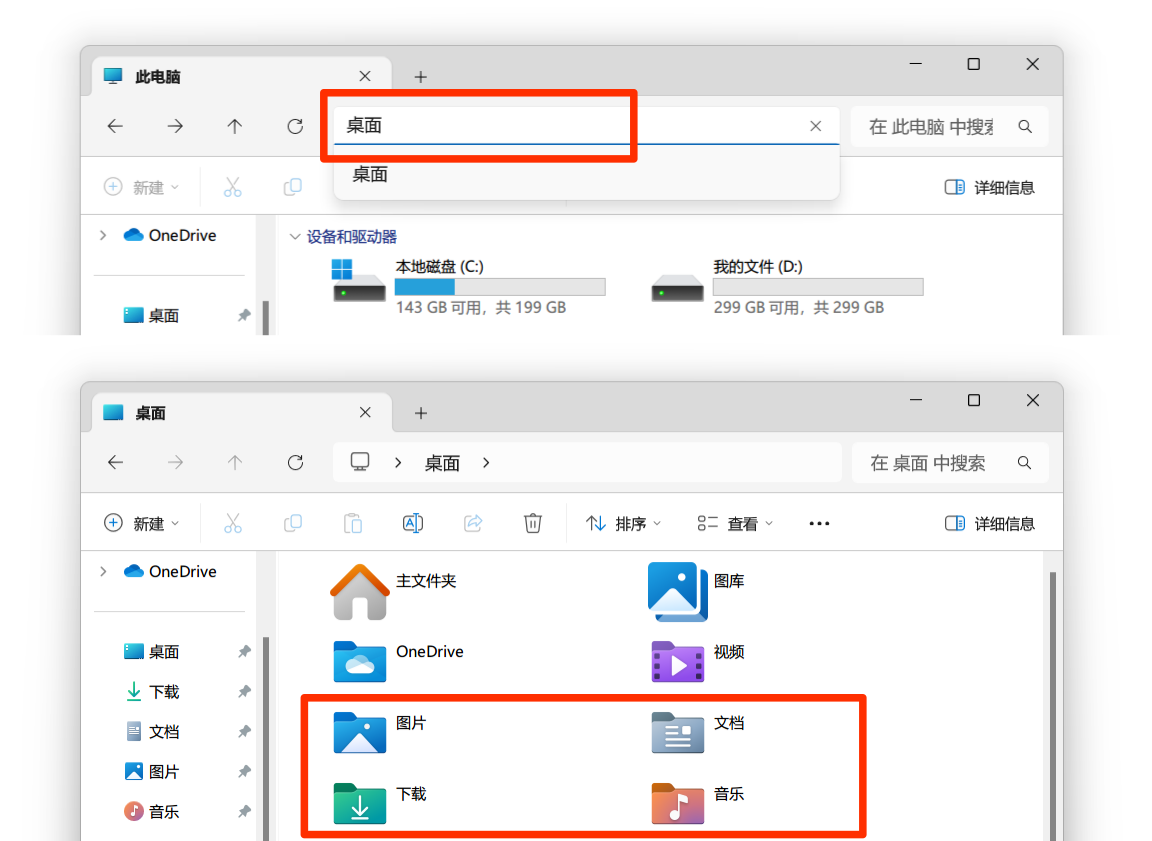
\includegraphics[width=.7\textwidth]{assets/basic/Reach_known_folders_manually.png}
  \caption{手动找到已知文件夹}
  \label{fig:Reach_known_folders_manually}
\end{figure}

而在 Windows 10 中,双击桌面上的【此电脑】,展开【文件夹】折叠项看到这些文件夹,如\autoref{fig:User_directories}。

\begin{figure}[htb!]
  \centering
  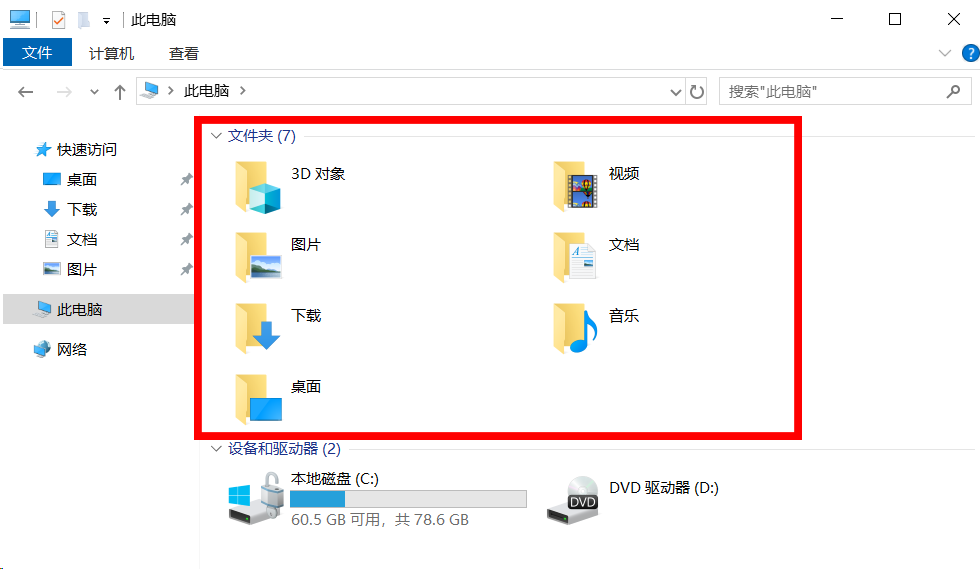
\includegraphics[width=.7\textwidth]{assets/basic/User_directories.png}
  \caption{Windows 10 的已知文件夹}
  \label{fig:User_directories}
\end{figure}

默认情况下,\cprotect\regcolor{已知文件夹的实际位置在 \MissingVerb{C:\用户\<你的用户名>},这是你的「用户配置文件夹」(User Profile Folder,俗称「用户文件夹」)。}除了直接在【此电脑】中查看外,你也可以手动打开这个路径来找到它们。已知文件夹涵盖了「桌面」「文档」「图片」「音乐」「视频」等多种类别,并且都配有形象的图标。如果你计划将自己的文件存放在 C 盘,这些目录是不错的选择:毕竟,C 盘作为 Windows 的系统分区,有严格的保护机制,最好不要把你的文件直接放在 C 盘根目录下。

但如果你打算把自己的文件放到其他的分区,你的选择就会自由很多,各个分区的根目录也许是不错的位置。你可以仿照 Windows 给你的已知文件夹,自己在其他分区的根目录下按类别新建好「文档」「电影」「音频」等文件夹,用来帮助自己整理文件。或者更直接点,\regcolor{你还可以将 Windows 提供给你的这些已知文件夹迁移到其他分区},这样它们的实际位置就不再是 \MissingVerb{C:\用户\<你的用户名>},而是你选定的地方了。例如,如果你想使用 D 盘根目录即 \MissingVerb{D:\} 来存放这些已知文件夹,可以按下面的步骤操作。

\begin{warning}
  如果你的电脑登录了 OneDrive(微软推出的云同步盘),并且针对文档、图片等已知文件夹启用了备份功能,那么它们可能已经被迁移到了你的 OneDrive 文件夹下。默认情况下它是 \MissingVerb{C:\用户\<你的用户名>\OneDrive}。\regcolor{此时,你很可能无法再按后文的步骤,将它们迁移到其他地方。}

  若你曾把某些软件安装在了已知文件夹下(如「文档」或「桌面」里面——不是快捷方式,是软件本体在里面),那么\regcolor{按下文的步骤迁移对应的已知文件夹后,那些软件可能无法正常使用}。

  许多软件都在利用已知文件夹存储数据,但它们内部记录的是已知文件夹的完整路径(例如 QQ 使用 \MissingVerb{C:\用户\<你的用户名>\文档})。即使你迁移了已知文件夹,它们仍会按照原来的路径存储文件。所以,一旦迁移完成,你得手动打开相应软件更改数据存储位置。
\end{warning}

\begin{itemize}
  \item 在资源管理器中,右击某个我们想要迁移的文件夹(比如【文档】),选择【属性】,然后切换到【位置】选项卡,如\autoref{fig:Pos_of_Documents}。
    \begin{figure}[htb!]
      \centering
      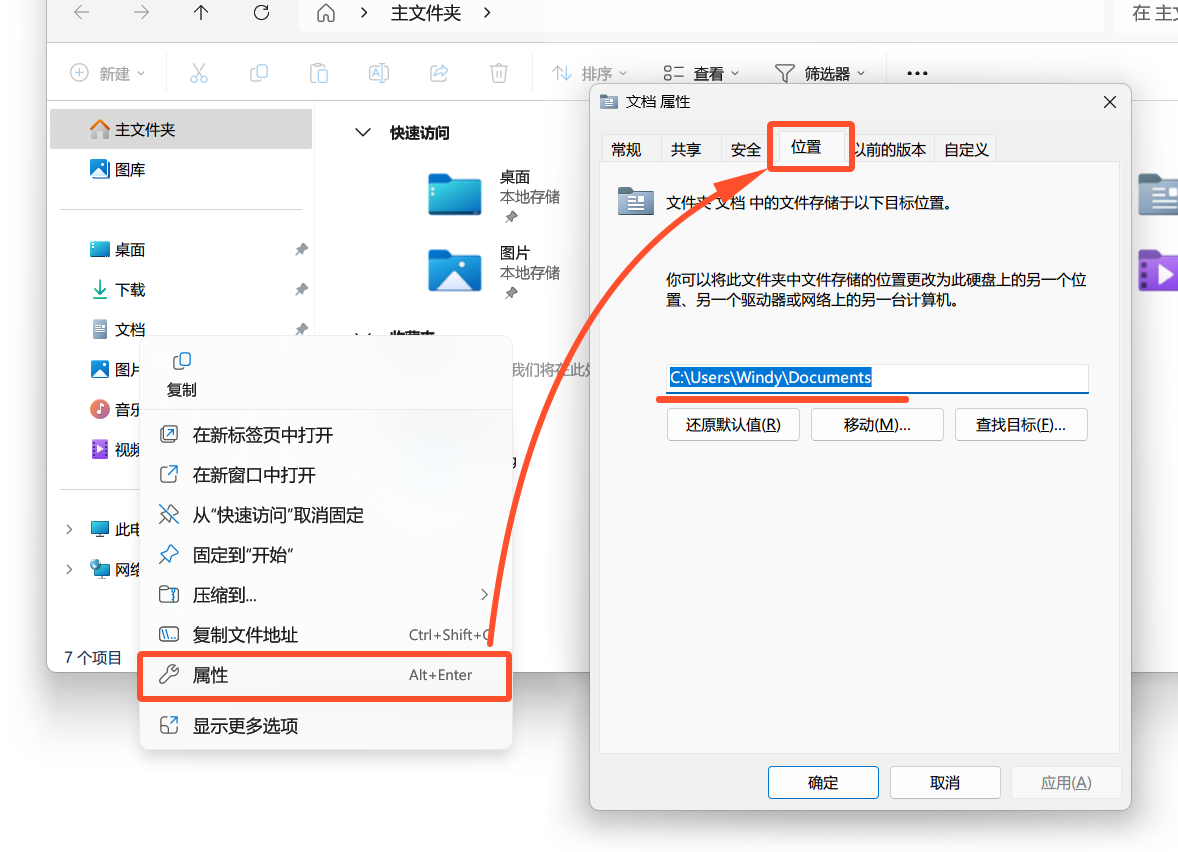
\includegraphics[width=.7\textwidth]{assets/basic/Pos_of_Documents.png}
      \caption{查看「文档」的位置}
      \label{fig:Pos_of_Documents}
    \end{figure}
  \item 我们将此处文本框中内容的 \MissingVerb{C:\Users\<你的用户名>\}这一部分\cprotect\regcolor{(注意:最后一个 \MissingVerb{Documents} 之类的名字不要动!)}\footnote{如果你不小心把一个已知文件夹的位置设置成了某个磁盘的根目录(比如说\MissingTT{D:\textbackslash}),可能很难再改回来。}改成 \MissingVerb{D:\}。\regcolor{也就是说,对于「文档」而言,改完之后的完整路径是:}
    \begin{MissingVerbatim}
      D:\Documents
    \end{MissingVerbatim}
  \item 点击【应用】,提示「文件夹 ‘\MissingVerb{D:\Desktop}’ 不存在,是否新建该文件夹」,选择【是】。
  \item 紧接着提示「是否要将所有文件从原位置移动到新位置」,选择【是】。
\end{itemize}

一般来说移动操作很快就会完成。完成后,点击【确定】。这样「文档」文件夹就被成功地迁移到了 D 盘,你可以直接在【此电脑】中双击【文档】打开它,也可以打开 \MissingVerb{D:\文档} 来访问,如\autoref{fig:Moved_user_directories} 所示。\regcolor{如果你打算使用 C 盘以外的分区存放自己的文件,我们强烈建议你迁移各已知文件夹到对应的分区},因为它们能帮你更好地管理文件。

\begin{figure}[htb!]
  \centering
  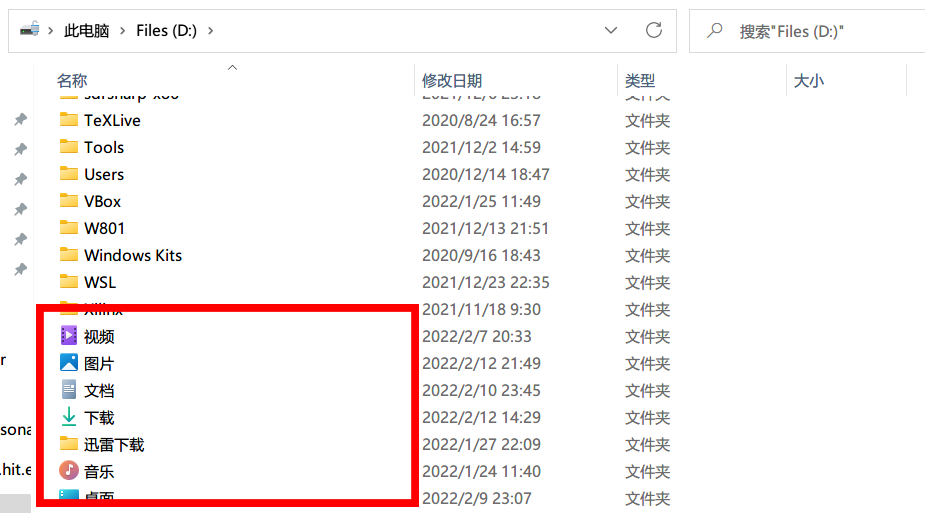
\includegraphics[width=.7\textwidth]{assets/basic/Moved_user_directories.png}
  \caption{移走的已知文件夹}
  \label{fig:Moved_user_directories}
\end{figure}

在找到合适的位置后,我们便可以建立一套自己的分类方法来对文件进行整理和分类。

\begin{itemize}
  \item 例如你有一些「学习资源」,你便可以合适的地方建立一个名为「学习资源」的文件夹,再在其下——无论是按学科(例如「高数」「线代」「物理」),还是按时间(例如「大一上」「大一下」)——建立更多的子文件夹,来为它们进行更为详尽的分类。
  \item 再例如你有许多「大片」,你也可以按照地区、上映时间甚至是主演什么的为它们分类。不过鉴于大片不仅是名气大,占用空间也大,我们推荐腾出一个分区(甚至是一块硬盘)来存放它们。
\end{itemize}

总之,「\regcolor{为你的文件进行合理分类}」与「\regcolor{将你的硬盘进行合理分配}」便是这里的核心思想。

\subsection{定期打扫}

电脑里面的东西总是随着我们的日常使用而越积越多\CJKsout*{(比如微软的更新,一更一大堆;以及 QQ、微信的文件接收文件夹,相信你不一定知道在哪\footnotemark)},\footnotetext{你可以先把一个文件发给自己,然后删掉原始文件,再下回来,就能找到这些接收文件夹的位置(真是曲线救国啊)。}所以定期检查你不需要的东西然后扔掉它们显得尤为重要。

对于系统分区 C 盘来说,你不去动它,它也会被塞入一些诸如系统临时文件、Windows 更新文件等等这些。诸如「火绒安全软件」「360 电脑管家」之类的工具通常都会提供「系统清理」功能,可以帮助你清理这些文件。除此之外,Windows 自身也提供了一个磁盘清理工具。在\chapref{cha:manage-storage} 一章中,你将学习到如何使用它来打扫你的 C 盘。

上述各种磁盘清理工具并不会把我们日常中积累的用户文件(例如你收到的课件、文档等)也清理掉,但在日常使用过程中,我们也会不可避免地产生许许多多的冗余文件,或是曾经需要而现在不再需要的文件。这里不妨就来看看你的「下载」文件夹:

\begin{itemize}
  \item 作为一个已知文件夹,它默认在 C 盘,如果你没有按照前文迁移它的话。各大浏览器、新版 QQ、飞书等应用都会把接收到、下载到的文件存在这里;
  \item 点击资源管理器左侧的【下载】,进入 \MissingTT{下载} 文件夹,将其中的所有文件检查一遍,有用的就如上文所述——无论按时间也好还是按类型也好——归类、无用的则直接删除,这就大功告成了;
  \item 进一步而言,如果你不想让各大软件都往 C 盘的这里塞东西,可以参照前文的方法将它迁走,或者在各个应用中设置默认下载文件的存储路径到你喜欢的地方。
\end{itemize}

\begin{note}
  这也解释了为什么我们在前文中提到,如果你决定使用其他分区存放文件,就最好将这些已知文件夹一并迁移。因为根据微软的规范,许多软件都会默认使用它们来存放数据,将它们迁移走可以更好地缓解 C 盘压力。
\end{note}

同样地,在你已经归好类的文件体系中,也要时不时进行检查,删去冗余与无用文件,这样能够保持你的文件系统简而精。《礼记·大学》载:「苟日新,日日新,又日新。」如是而已。

\practice

\begin{enumerate}
  \item 查看自己电脑的几个分区的「卷标」,并依照自己的文件分类习惯修改成自己所喜欢的名字。例如,叫「资料」或者「Files」就比「新加卷」或者没有卷标(会显示「本地磁盘」)要直观得多。
  \item 尝试把一个图片文件的扩展名改成 \MissingVerb{txt},然后用「记事本」打开它。你看到了什么?\CJKunderline*{记得改回来哦!}
  \item 试着根据我们的建议,选择合适的分区运用策略。如果需要,可以试试迁移一部分已知文件夹。
    \begin{warning}
      注意迁移的时候千万看清楚目标路径是完整的 \MissingVerb{D:\Documents}、\MissingVerb{D:\Desktop} 这样的路径,而不是光秃秃的一个 \MissingVerb{D:\}。
    \end{warning}
  \item 整理你的「下载」文件夹。
  \item 选择你自己的几个文件和文件夹,把它们打包成一个压缩文件 \MissingVerb{MyArchive.zip},复制到其他的某个地方,尝试两种不同的解压方式「解压到当前位置」「解压到 \MissingVerb{MyArchive\}」。
  \item 创建一个文档(可以是纯文本文件 \MissingVerb{txt} 或者 Word 文档 \MissingVerb{docx} 等)并写入一些内容,然后制作它的两个快捷方式,并把这两个快捷方式放在两个与源文件都不一样的地方。试着双击打开那两个快捷方式,你发现了什么?删掉两个快捷方式中的一个,源文件被删除了吗?另一个快捷方式还在吗?
\end{enumerate}